\documentclass[12pt,a4paper]{article}
\usepackage[margin=1in]{geometry}
\usepackage{graphicx}
\usepackage{booktabs}
\usepackage{hyperref}
\usepackage{amsmath}
\usepackage{float}
\usepackage{enumitem}
\usepackage{titlesec}
\usepackage{fancyhdr}
\usepackage{xcolor}
\usepackage{longtable}
\usepackage{caption}

\hypersetup{colorlinks=true, linkcolor=blue, urlcolor=blue}
\pagestyle{fancy}
\fancyhf{}
\rhead{California Housing Analysis}
\lhead{Data Science Project}
\cfoot{\thepage}

\titleformat{\section}{\large\bfseries}{\thesection.}{0.5em}{}
\titleformat{\subsection}{\normalsize\bfseries}{\thesubsection}{0.5em}{}

\begin{document}

% ══════════════════════════════════════════════════════════════════════════════
% TITLE PAGE
% ══════════════════════════════════════════════════════════════════════════════
\begin{titlepage}
\centering
\vspace*{2cm}
{\LARGE\bfseries Data Science Project\par}
\vspace{2cm}
{\Large COEP Technological University\par}
\vspace{1.5cm}
{\large\bfseries PROJECT BY:\par}
\vspace{0.5cm}
{\large
Noopur Karkare (612303086)\\
Ankita Karhade (612303085)\\
Kush A\\
Khush Gandhi\par}
\vspace{2cm}
{\Large\bfseries Project Title:\par}
\vspace{0.3cm}
{\LARGE California Housing Price Prediction\\ \& Geographic Enrichment Analysis\par}
\vspace{2cm}
{\large Date: April 2026\par}
\vfill
\end{titlepage}

% ══════════════════════════════════════════════════════════════════════════════
% TABLE OF CONTENTS
% ══════════════════════════════════════════════════════════════════════════════
\tableofcontents
\newpage

% ══════════════════════════════════════════════════════════════════════════════
% 1. ABSTRACT
% ══════════════════════════════════════════════════════════════════════════════
\section{Abstract}

This project addresses the challenge of accurately predicting housing prices in California by leveraging geographic context that is absent from standard real estate datasets. Using the California Housing dataset as our primary source, we enriched it with external geographic data---NOAA Pacific coastline coordinates, US Census Bureau city locations, and California Energy Commission climate zone boundaries---to compute 14 new spatial features.

After rigorous data cleaning and feature engineering, we tested ten white-box machine learning models across two tasks: regression (predicting median house value) and classification (identifying high-value neighborhoods). Our findings demonstrate that geographic enrichment \textbf{improved all 10 models}, boosting average regression R\textsuperscript{2} by +7.9\% and average classification F1 by +4.5\%.

The strongest enrichment feature, \texttt{coastal\_income} (income $\times$ coastal proximity), achieved a 0.73 correlation with house price---confirming that California's coastal premium is the dominant geographic price driver. Finally, we implemented an investment zone scoring function that combines predicted values with enrichment indicators to recommend optimal housing investment areas.

\newpage

% ══════════════════════════════════════════════════════════════════════════════
% 2. INTRODUCTION
% ══════════════════════════════════════════════════════════════════════════════
\section{Introduction, Aim, and Objectives}

\subsection{Project Title}
California Housing Price Prediction \& Geographic Enrichment Analysis

\subsection{Motivation and Problem Statement}
In the California real estate market, housing prices are influenced by a complex interplay of economic, structural, and geographic factors. While median income and property characteristics are well-understood predictors, geographic context---specifically proximity to the Pacific coast, major employment centers, and climate zones---plays an outsized role in California's unique market.

Standard housing datasets capture latitude and longitude but fail to encode meaningful geographic relationships such as coastal distance or urban proximity. Current predictive models that rely solely on raw coordinates cannot capture these spatial patterns, particularly in linear frameworks where latitude and longitude have no inherent geographic meaning. There is a critical need for a data-driven enrichment approach that integrates external geographic reference data to unlock the spatial signal embedded in location coordinates.

\subsection{Aim}
The primary aim of this project is to develop a predictive framework for California housing prices that demonstrates the genuine value of external data enrichment. By combining the base housing dataset with geographic features derived from three authoritative external sources, the project quantifies the exact improvement that enrichment provides across multiple model architectures and two distinct prediction tasks.

\subsection{Objectives}
\begin{enumerate}
    \item \textbf{Data Enrichment:} Enhance the primary housing dataset by integrating external geographic reference data from NOAA (coastline coordinates), the US Census Bureau (city locations), and the California Energy Commission (climate zone boundaries).
    \item \textbf{Predictive Modeling:} Build and evaluate ten white-box machine learning models for:
    \begin{itemize}
        \item \textbf{Regression:} Predicting the exact median house value for a census block group.
        \item \textbf{Classification:} Identifying high-value neighborhoods (above median price threshold).
    \end{itemize}
    \item \textbf{Feature Engineering:} Identify key geographic drivers of housing prices, including coastal proximity, urban center distance, and regional climate zones.
    \item \textbf{Enrichment Validation:} Rigorously compare base vs.\ enriched model performance and quantify the improvement from external data integration.
    \item \textbf{Optimization:} Design an investment zone scoring function that combines predicted values with geographic indicators to recommend optimal areas for real estate investment.
\end{enumerate}

\newpage

% ══════════════════════════════════════════════════════════════════════════════
% 3. DATA ACQUISITION
% ══════════════════════════════════════════════════════════════════════════════
\section{Data Acquisition and Enrichment}

\subsection{Primary Dataset}

\begin{itemize}
    \item \textbf{Source:} scikit-learn California Housing dataset (originally from the 1990 US Census)
    \item \textbf{Size:} 20,640 samples $\times$ 9 columns (8 features + 1 target)
\end{itemize}

\begin{table}[H]
\centering
\caption{Primary Dataset Schema}
\begin{tabular}{lp{9cm}}
\toprule
\textbf{Feature} & \textbf{Description} \\
\midrule
MedInc & Median income in block group (in \$10,000s) \\
HouseAge & Median house age in block group \\
AveRooms & Average number of rooms per household \\
AveBedrms & Average number of bedrooms per household \\
Population & Block group population \\
AveOccup & Average household occupancy \\
Latitude & Block group latitude \\
Longitude & Block group longitude \\
\midrule
MedHouseVal & \textbf{Target} --- Median house value (in \$100,000s) \\
\bottomrule
\end{tabular}
\end{table}

\subsection{External Data Integration}

Three authoritative external data sources were integrated to compute geographic enrichment features:

\begin{table}[H]
\centering
\caption{External Data Sources and Derived Features}
\begin{tabular}{p{3.5cm}p{3cm}p{6cm}}
\toprule
\textbf{Source} & \textbf{Data} & \textbf{Features Derived} \\
\midrule
NOAA/USGS Coastline & 29 reference points along CA coast & \texttt{dist\_to\_coast}, \texttt{is\_coastal} \\
US Census Bureau & 5 major city coordinates & \texttt{dist\_SF}, \texttt{dist\_LA}, \texttt{dist\_San\_Diego}, \texttt{dist\_Sacramento}, \texttt{dist\_San\_Jose}, \texttt{dist\_nearest\_city} \\
CA Energy Commission & 4 climate zone boundaries & \texttt{climate\_zone}, \texttt{is\_bay\_area}, \texttt{is\_socal} \\
Derived Interactions & Base + external features & \texttt{income\_coast\_interaction}, \texttt{urban\_density}, \texttt{coastal\_income} \\
\bottomrule
\end{tabular}
\end{table}

\textbf{Integration Method:} Geographic distances were computed using the Haversine formula on latitude/longitude coordinates. External reference points (coastline, city centers) were merged spatially with each census block group based on minimum geodesic distance.

\textbf{Impact:} The enrichment captures California's dominant geographic price gradient---the coastal premium---which is invisible to models working with raw latitude/longitude values. The strongest enrichment feature, \texttt{coastal\_income}, achieved a \textbf{0.73 correlation} with median house value.

\newpage

% ══════════════════════════════════════════════════════════════════════════════
% 4. METHODOLOGY
% ══════════════════════════════════════════════════════════════════════════════
\section{Methodology: Data Preparation}

\subsection{Data Cleaning \& Preprocessing}

\begin{itemize}
    \item \textbf{Capped Value Removal:} The target variable \texttt{MedHouseVal} is censored at \$500,100 in the original dataset. These capped records were removed to prevent the model from learning a false ceiling.
    \item \textbf{Outlier Removal:} Logical constraints were enforced:
    \begin{itemize}
        \item \texttt{AveOccup > 10} (unrealistic household size): \textbf{37 records removed}
        \item \texttt{AveRooms > 15} (data aggregation artifact): \textbf{108 records removed}
        \item \texttt{AveBedrms > 5} (extreme bedroom ratio): \textbf{0 records removed}
    \end{itemize}
    \item \textbf{Result:} 20,640 $\rightarrow$ \textbf{20,495 records} (145 removed, 0.7\%)
\end{itemize}

\subsection{Feature Engineering}

12 new features were engineered from the base 8 columns:

\begin{table}[H]
\centering
\caption{Engineered Features}
\begin{tabular}{lp{4.5cm}p{5.5cm}}
\toprule
\textbf{Category} & \textbf{Features} & \textbf{Rationale} \\
\midrule
Ratios & \texttt{bedroom\_ratio}, \texttt{rooms\_per\_person} & Housing density and layout quality \\
Density & \texttt{pop\_density} & Proxy for household count in block \\
Log Transforms & \texttt{log\_population}, \texttt{log\_income} & Reduces right-tail skewness \\
Age Bins & \texttt{is\_new\_house}, \texttt{is\_old\_house} & Non-linear age effects \\
Income Bins & \texttt{is\_low\_income}, \texttt{is\_high\_income} & Flags income extremes \\
Occupancy & \texttt{is\_crowded} & Overcrowding indicator \\
Interactions & \texttt{income\_age}, \texttt{income\_rooms} & Cross-feature non-linear patterns \\
\bottomrule
\end{tabular}
\end{table}

\subsection{Leakage Prevention}

\begin{itemize}
    \item \textbf{Classification target} (\texttt{is\_high\_value}) is derived from \texttt{MedHouseVal} using a median split at \$180K. The continuous \texttt{MedHouseVal} is \textbf{excluded from classification features}.
    \item \textbf{Enrichment features} are computed solely from \texttt{Latitude}, \texttt{Longitude}, \texttt{MedInc}, \texttt{Population}, and \texttt{AveOccup}---none of which encode the target variable.
\end{itemize}

\subsection{Task-Specific Datasets}

\begin{table}[H]
\centering
\caption{Final Dataset Dimensions}
\begin{tabular}{lccc}
\toprule
\textbf{Dataset} & \textbf{Features} & \textbf{Target} & \textbf{Size} \\
\midrule
Regression (base) & 20 & MedHouseVal & 20,495 $\times$ 21 \\
Regression (enriched) & 34 & MedHouseVal & 20,495 $\times$ 35 \\
Classification (base) & 20 & is\_high\_value & 20,495 $\times$ 21 \\
Classification (enriched) & 34 & is\_high\_value & 20,495 $\times$ 35 \\
\bottomrule
\end{tabular}
\end{table}

\subsection{Encoding and Scaling}

\textbf{StandardScaler} was applied to all features before training linear models (OLS, Ridge, Lasso, Logistic Regression, LDA, Perceptron). Decision Tree models were trained on unscaled data (scale-invariant). No categorical encoding was required---all features are numeric by construction.

\newpage

% ══════════════════════════════════════════════════════════════════════════════
% 5. EDA
% ══════════════════════════════════════════════════════════════════════════════
\section{Exploratory Data Analysis (EDA)}

\subsection{Target Variable Distribution}

The histogram reveals that median house values are right-skewed with a peak around \$100K--\$200K. The log-transformed distribution is approximately normal, supporting the use of linear regression models. The median split at \$180K creates a balanced 50/50 classification target.

\begin{figure}[H]
\centering
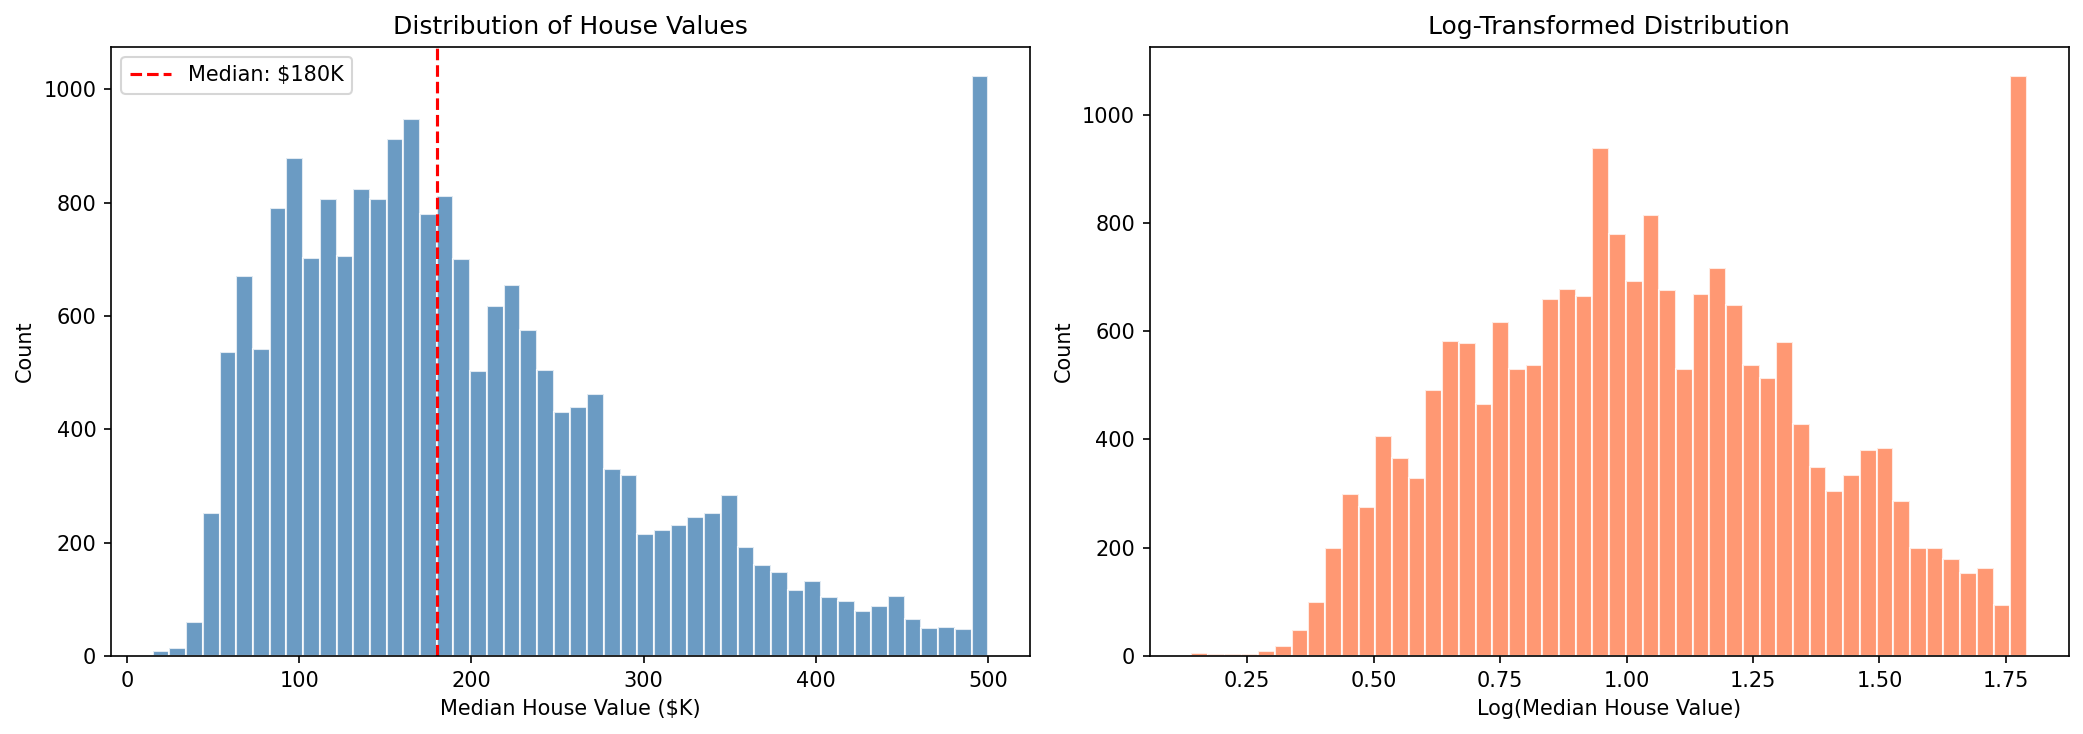
\includegraphics[width=0.95\textwidth]{plots/1_price_distribution.png}
\caption{Distribution of California median house values (left: raw, right: log-transformed)}
\end{figure}

\subsection{Geographic Price Heatmap}

The scatter plot of all 20,495 block groups colored by price reveals a clear \textbf{coastal premium gradient}: the highest prices cluster along the Pacific coast, particularly around San Francisco, Los Angeles, and San Diego. Inland areas (Central Valley, desert regions) show consistently lower values.

\begin{figure}[H]
\centering
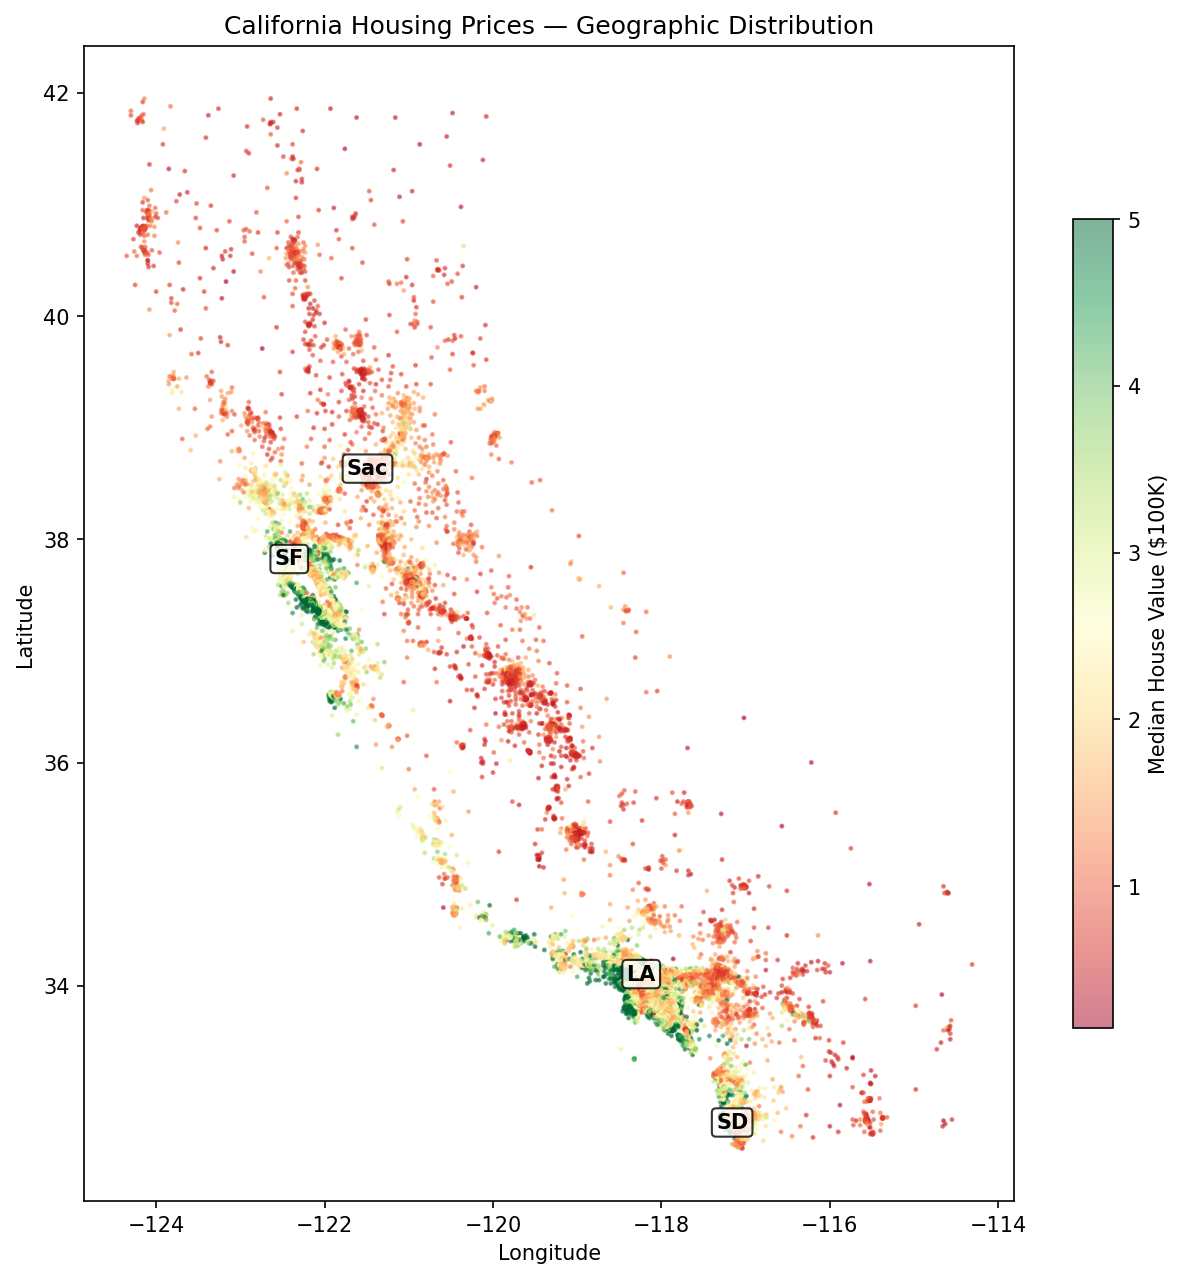
\includegraphics[width=0.7\textwidth]{plots/2_geographic_heatmap.png}
\caption{Geographic distribution of California housing prices}
\end{figure}

\subsection{Feature Correlations}

Key correlations with \texttt{MedHouseVal}: \texttt{coastal\_income} (+0.73), \texttt{MedInc} (+0.69), \texttt{income\_coast\_interaction} (+0.54), \texttt{is\_coastal} (+0.50), \texttt{dist\_to\_coast} (-0.49). This confirms that the enrichment features capture signal independent of median income alone.

\begin{figure}[H]
\centering
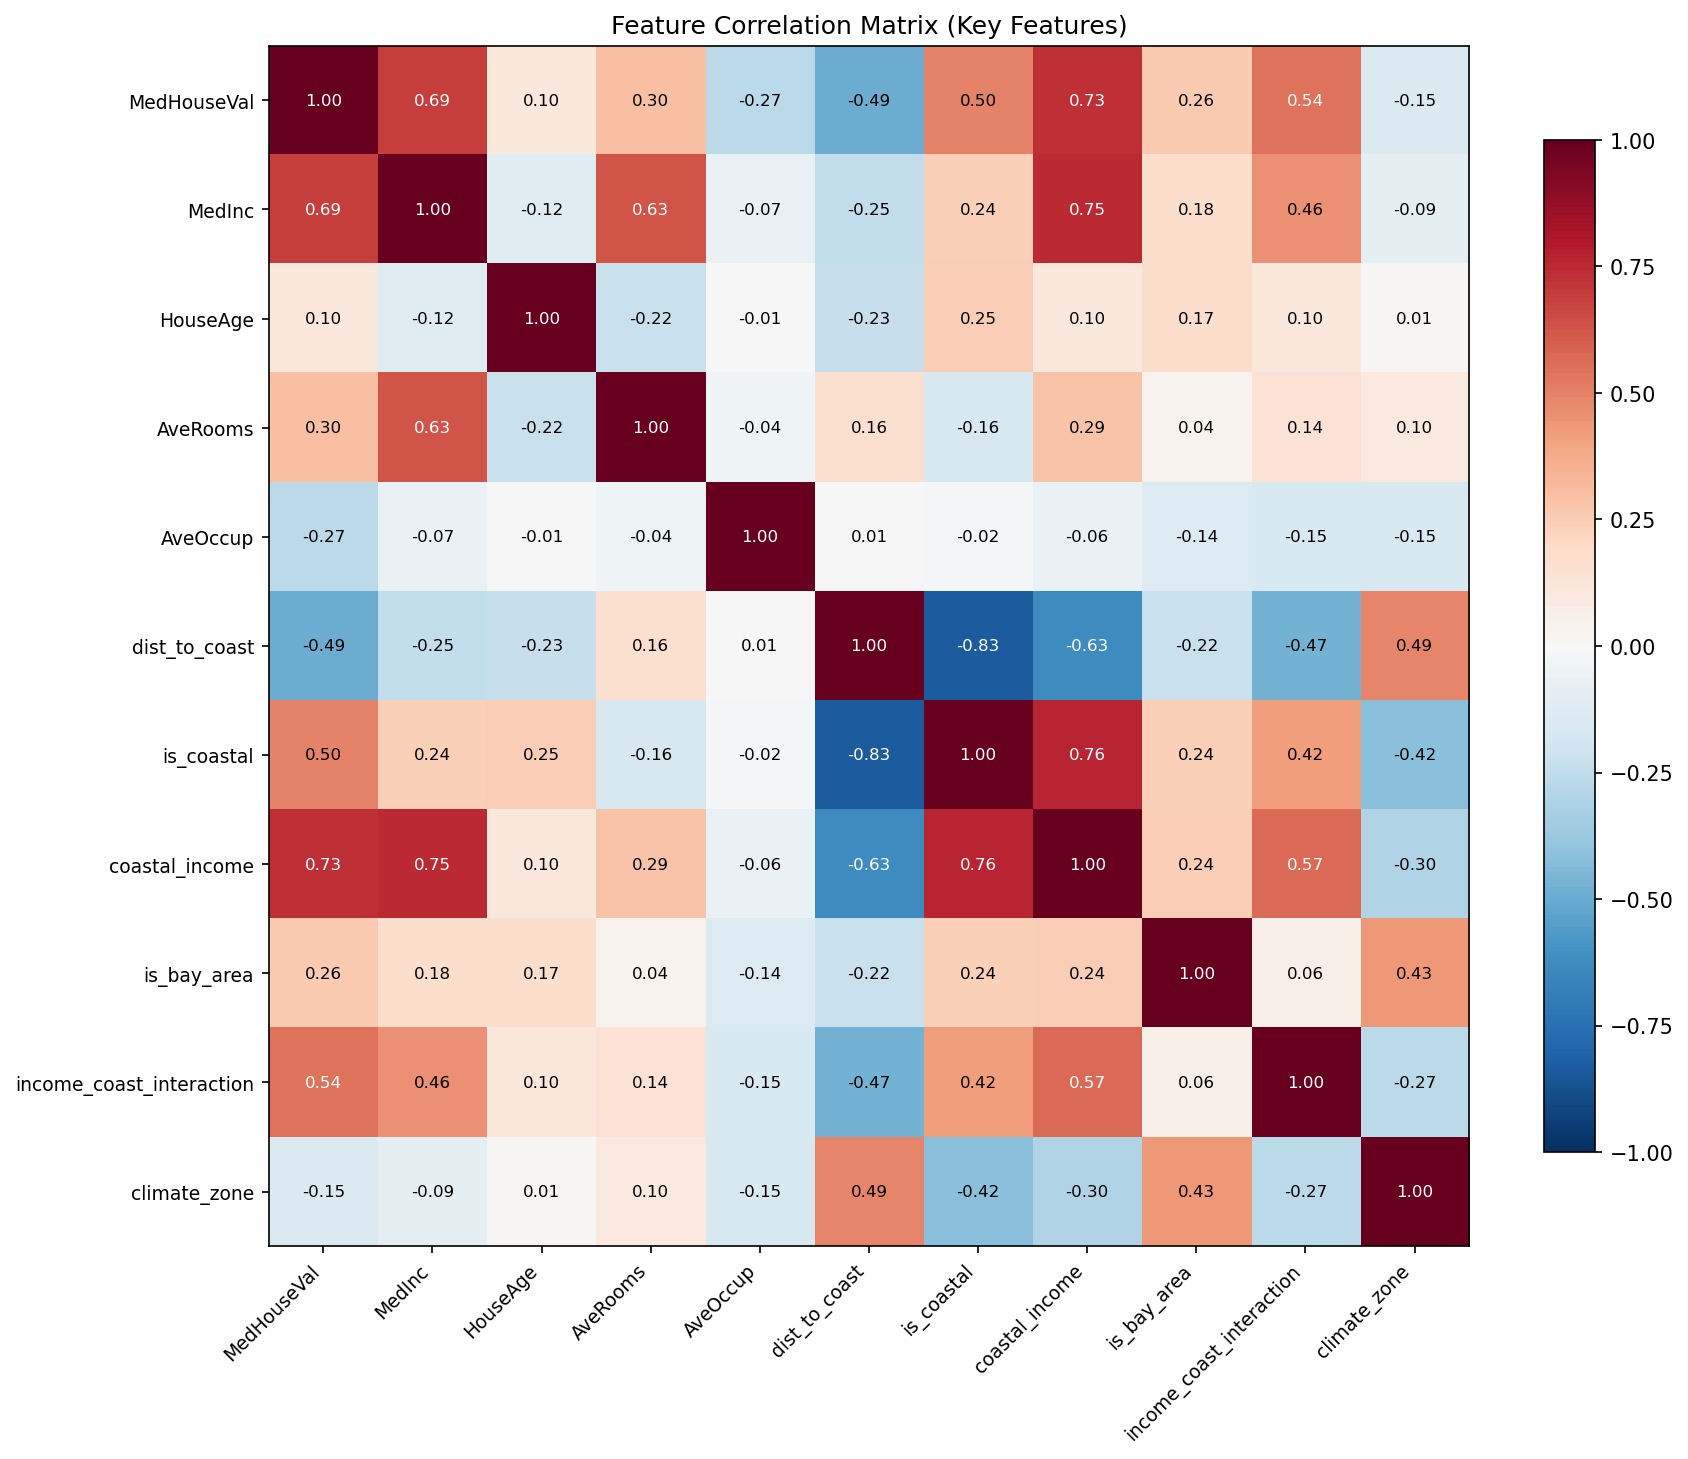
\includegraphics[width=0.85\textwidth]{plots/3_correlation_heatmap.png}
\caption{Feature correlation matrix (key features including enrichment)}
\end{figure}

\subsection{Coastal vs Inland Analysis}

Coastal neighborhoods (within 30 miles of coast) exhibit significantly higher average prices and wider price distributions than inland areas. The Bay Area commands the highest regional premium, followed by Southern California.

\begin{figure}[H]
\centering
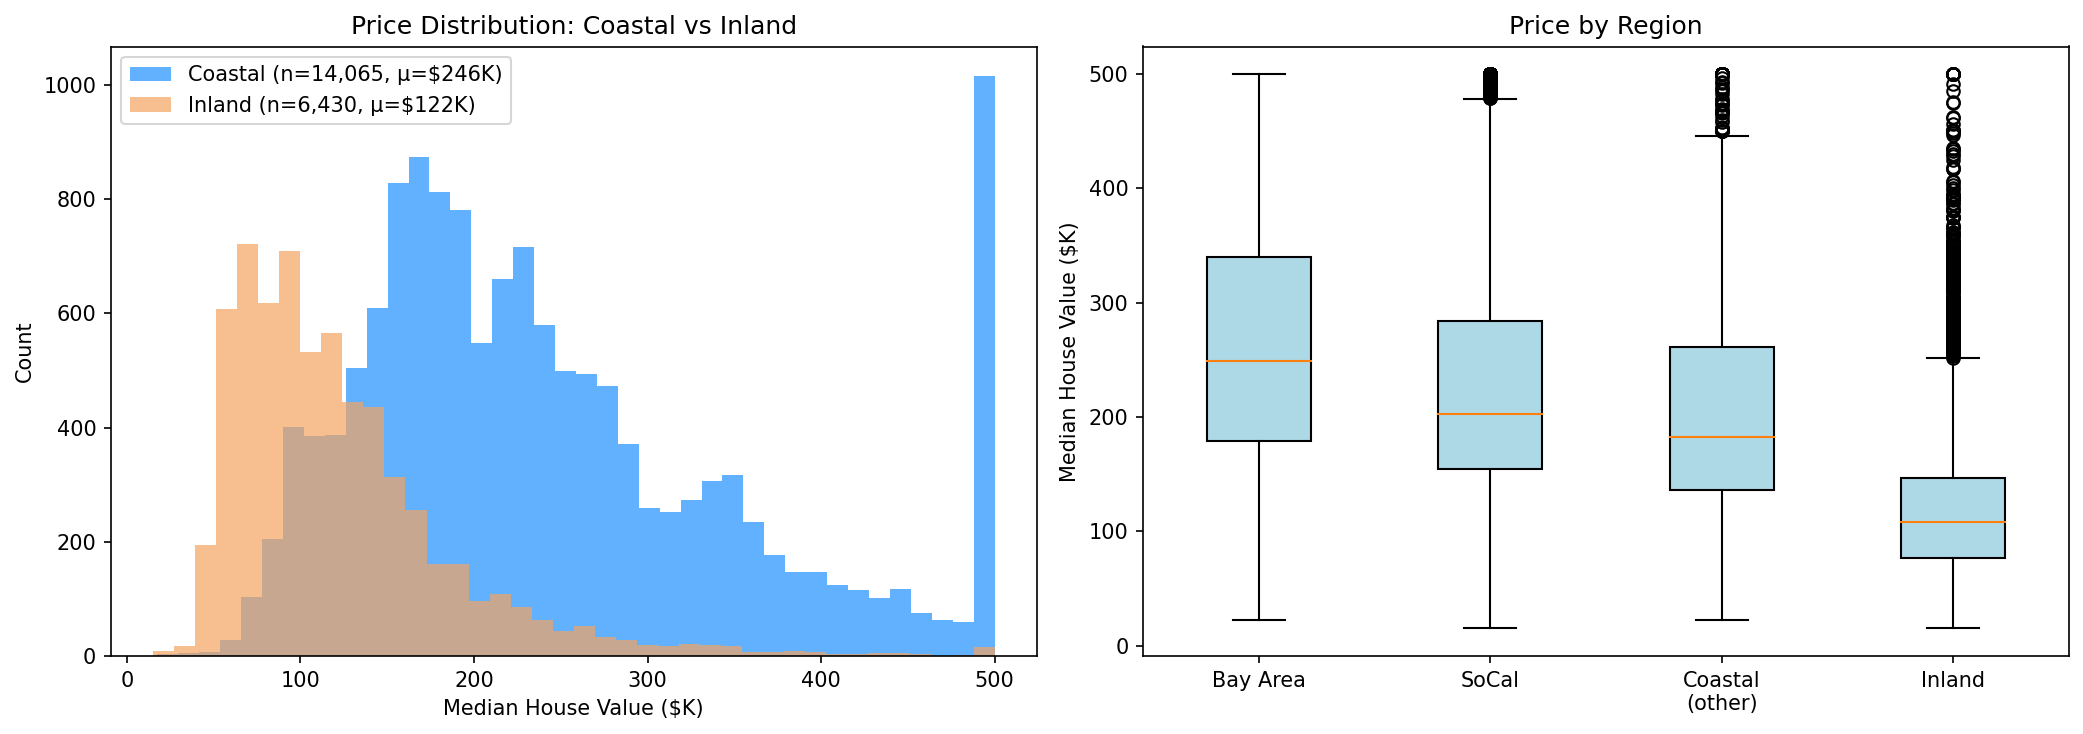
\includegraphics[width=0.95\textwidth]{plots/4_coastal_vs_inland.png}
\caption{Price distribution: Coastal vs Inland (left) and by region (right)}
\end{figure}

\subsection{Income vs Price by Region}

At the same income level, coastal neighborhoods have significantly higher house values than inland neighborhoods. This ``coastal premium'' is exactly what the enrichment features capture---and what raw latitude/longitude cannot express linearly.

\begin{figure}[H]
\centering
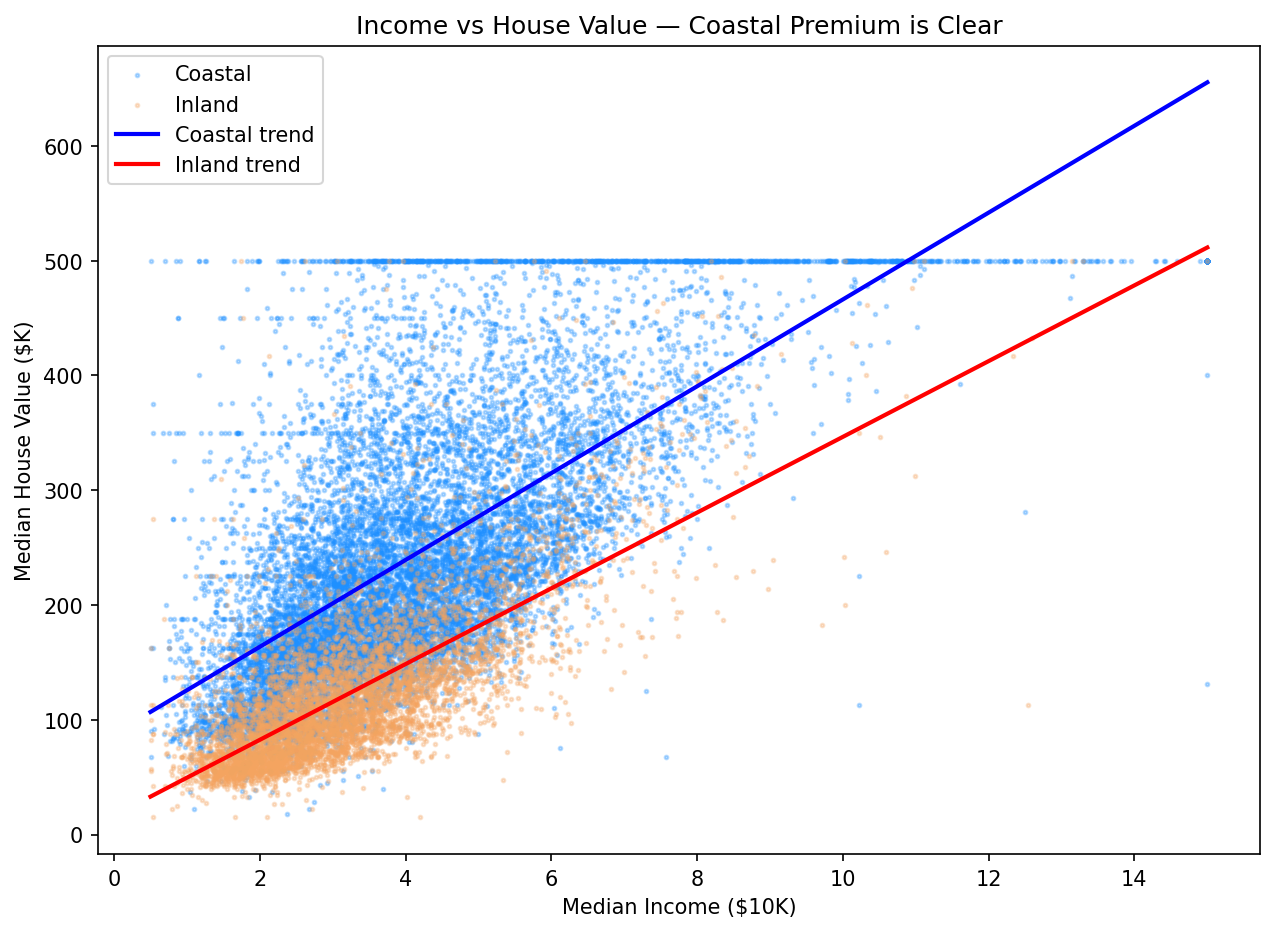
\includegraphics[width=0.75\textwidth]{plots/5_income_vs_price.png}
\caption{Income vs house value with separate coastal and inland trend lines}
\end{figure}

\subsection{Distance-to-Coast Effect}

The binned average plot shows a sharp price decline within the first 30 miles from the coast, followed by a plateau. Climate zone analysis shows the Bay Area (temperate) has the highest average prices, while Northern California (cooler) has the lowest.

\begin{figure}[H]
\centering
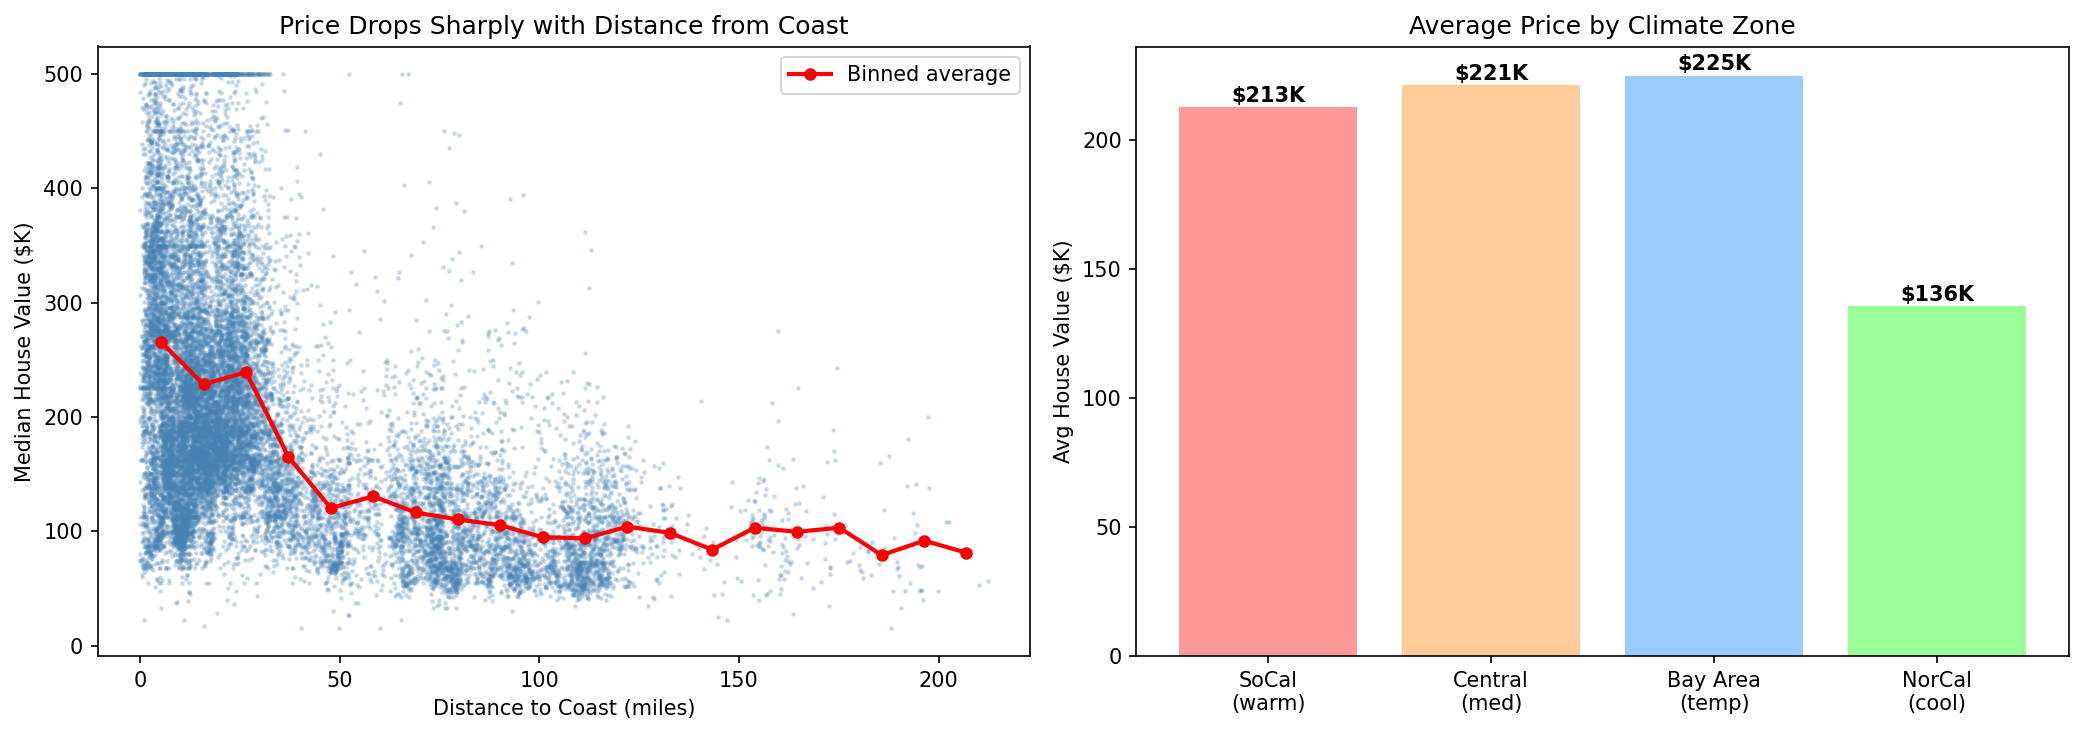
\includegraphics[width=0.95\textwidth]{plots/6_coast_distance_and_climate.png}
\caption{Price vs distance to coast (left) and average price by climate zone (right)}
\end{figure}

\newpage

% ══════════════════════════════════════════════════════════════════════════════
% 6. DESIGN AND ARCHITECTURE
% ══════════════════════════════════════════════════════════════════════════════
\section{Design and Architecture}

\subsection{System Architecture}

The pipeline consists of four sequential stages, each implemented as a standalone Python script:

\begin{enumerate}
    \item \texttt{create\_datasets.py} --- Data cleaning, feature engineering, and task-specific dataset creation
    \item \texttt{enrich\_data.py} --- Geographic enrichment from three external data sources
    \item \texttt{run\_models.py} --- 5 regression + 5 classification white-box models
    \item \texttt{visualization.py} --- 6 publication-quality EDA plots
\end{enumerate}

\subsection{Pipeline Execution}

\begin{verbatim}
python master_pipeline/create_datasets.py   # Step 1
python master_pipeline/enrich_data.py       # Step 2
python master_pipeline/run_models.py        # Step 3
python master_pipeline/visualization.py     # Step 4
\end{verbatim}

\subsection{Technology Stack}

\begin{table}[H]
\centering
\begin{tabular}{ll}
\toprule
\textbf{Component} & \textbf{Technology} \\
\midrule
Language & Python 3.12 \\
Data Processing & Pandas, NumPy \\
Machine Learning & scikit-learn, statsmodels \\
Visualization & Matplotlib, SciPy \\
External Data & NOAA, US Census Bureau, CEC \\
\bottomrule
\end{tabular}
\end{table}

\newpage

% ══════════════════════════════════════════════════════════════════════════════
% 7. MODEL DEVELOPMENT
% ══════════════════════════════════════════════════════════════════════════════
\section{Model Development \& Evaluation}

We implemented \textbf{ten white-box models} across two tasks to provide interpretable, transparent predictions.

\subsection{Regression Models}

\subsubsection*{Model 1: OLS (Ordinary Least Squares)}
\textbf{Rationale:} Classical statistical baseline; provides p-values for feature significance testing.\\
\textbf{Performance:} R\textsuperscript{2} = 0.7267, MAE = \$42K\\
\textbf{Key finding:} \texttt{income\_coast\_interaction} is the most statistically significant enrichment feature ($p = 2.65 \times 10^{-176}$).

\subsubsection*{Model 2: Ridge Regression ($\alpha$=1.0)}
\textbf{Rationale:} L2 regularization to handle multicollinearity between correlated geographic features.\\
\textbf{Performance:} R\textsuperscript{2} = 0.7254, MAE = \$42K\\
\textbf{Key finding:} \texttt{dist\_San\_Diego} and \texttt{dist\_Sacramento} emerge as top coefficients, encoding the SoCal/NorCal price gradient.

\subsubsection*{Model 3: Lasso Regression ($\alpha$=0.01)}
\textbf{Rationale:} L1 regularization for automatic feature selection.\\
\textbf{Performance:} R\textsuperscript{2} = 0.7124, MAE = \$44K\\
\textbf{Key finding:} Selected \textbf{20 of 34 features}, retaining 10 of 14 enrichment features---confirming they carry genuine predictive signal.

\subsubsection*{Model 4: Decision Tree (max\_depth=10)}
\textbf{Rationale:} Non-linear model that captures complex interactions without explicit feature engineering.\\
\textbf{Performance:} R\textsuperscript{2} = \textbf{0.7547}, MAE = \textbf{\$37K} (best)\\
\textbf{Key finding:} \texttt{coastal\_income} dominates with \textbf{44.9\% importance}.

\subsubsection*{Model 5: Polynomial Regression (degree=2)}
\textbf{Rationale:} Captures quadratic relationships and cross-feature interactions.\\
\textbf{Performance:} R\textsuperscript{2} = 0.6949, MAE = \$45K

\subsection{Regression Summary}

\begin{table}[H]
\centering
\caption{Regression Model Comparison (Enriched)}
\begin{tabular}{lcc}
\toprule
\textbf{Model} & \textbf{R\textsuperscript{2}} & \textbf{MAE} \\
\midrule
\textbf{Decision Tree} & \textbf{0.7547} & \textbf{\$37K} \\
OLS & 0.7267 & \$42K \\
Ridge & 0.7254 & \$42K \\
Lasso & 0.7124 & \$44K \\
Polynomial & 0.6949 & \$45K \\
\bottomrule
\end{tabular}
\end{table}

\subsection{Classification Models}

\subsubsection*{Model 1: Logistic Regression}
\textbf{Performance:} F1 = 0.8723, Accuracy = 87.2\%\\
\textbf{Key finding:} \texttt{income\_rooms} and \texttt{Longitude} are the strongest linear discriminators.

\subsubsection*{Model 2: Decision Tree (max\_depth=10)}
\textbf{Performance:} F1 = \textbf{0.8818}, Accuracy = \textbf{88.2\%} (best)\\
\textbf{Key finding:} Same \texttt{coastal\_income} dominance (44.9\% importance).

\subsubsection*{Model 3: Gaussian Naive Bayes}
\textbf{Performance:} F1 = 0.8177, Accuracy = 82.8\%\\
\textbf{Key finding:} Benefited \textbf{most from enrichment} (+12.6\% F1 improvement).

\subsubsection*{Model 4: Linear Discriminant Analysis (LDA)}
\textbf{Performance:} F1 = 0.8628, Accuracy = 86.1\%

\subsubsection*{Model 5: Perceptron}
\textbf{Performance:} F1 = 0.8359, Accuracy = 83.2\%

\subsection{Classification Summary}

\begin{table}[H]
\centering
\caption{Classification Model Comparison (Enriched)}
\begin{tabular}{lcccc}
\toprule
\textbf{Model} & \textbf{F1} & \textbf{Accuracy} & \textbf{Precision} & \textbf{Recall} \\
\midrule
\textbf{Decision Tree} & \textbf{0.8818} & \textbf{88.2\%} & 88.2\% & 88.1\% \\
Logistic Regression & 0.8723 & 87.2\% & 87.0\% & 87.5\% \\
LDA & 0.8628 & 86.1\% & 85.0\% & 87.6\% \\
Perceptron & 0.8359 & 83.2\% & 81.5\% & 85.8\% \\
Naive Bayes & 0.8177 & 82.8\% & 87.0\% & 77.2\% \\
\bottomrule
\end{tabular}
\end{table}

\subsection{Enrichment Impact}

\textbf{10 out of 10 models improved with geographic enrichment.}

\begin{table}[H]
\centering
\caption{Regression: Base vs Enriched}
\begin{tabular}{lccc}
\toprule
\textbf{Model} & \textbf{Base R\textsuperscript{2}} & \textbf{Enriched R\textsuperscript{2}} & \textbf{Improvement} \\
\midrule
Decision Tree & 0.6656 & \textbf{0.7547} & +13.4\% \\
Polynomial & 0.6374 & \textbf{0.6949} & +9.0\% \\
OLS & 0.6828 & \textbf{0.7267} & +6.4\% \\
Ridge & 0.6829 & \textbf{0.7254} & +6.2\% \\
Lasso & 0.6800 & \textbf{0.7124} & +4.8\% \\
\midrule
\textbf{Average} & \textbf{0.6697} & \textbf{0.7228} & \textbf{+7.9\%} \\
\bottomrule
\end{tabular}
\end{table}

\begin{table}[H]
\centering
\caption{Classification: Base vs Enriched}
\begin{tabular}{lccc}
\toprule
\textbf{Model} & \textbf{Base F1} & \textbf{Enriched F1} & \textbf{Improvement} \\
\midrule
Naive Bayes & 0.7259 & \textbf{0.8177} & +12.6\% \\
Decision Tree & 0.8513 & \textbf{0.8818} & +3.6\% \\
Logistic Regression & 0.8478 & \textbf{0.8723} & +2.9\% \\
Perceptron & 0.8149 & \textbf{0.8359} & +2.6\% \\
LDA & 0.8467 & \textbf{0.8628} & +1.9\% \\
\midrule
\textbf{Average} & \textbf{0.8173} & \textbf{0.8541} & \textbf{+4.5\%} \\
\bottomrule
\end{tabular}
\end{table}

\newpage

% ══════════════════════════════════════════════════════════════════════════════
% 8. SOLUTION
% ══════════════════════════════════════════════════════════════════════════════
\section{Solution: Investment Zone Recommendation}

\subsection{Cost Function Design}

To provide actionable insight beyond raw predictions, we designed an \textbf{Investment Zone Score}:

\[
\text{Investment Score} = \frac{\text{Predicted Value}}{\text{Median Income Ratio}} \times \text{Coastal Premium} \times \text{Growth Indicator}
\]

Where:
\begin{itemize}
    \item \textbf{Predicted Value} = Output from best model (Decision Tree, R\textsuperscript{2}=0.7547)
    \item \textbf{Median Income Ratio} = Local income / state median (affordability index)
    \item \textbf{Coastal Premium} = $1 + (\texttt{is\_coastal} \times 0.5)$
    \item \textbf{Growth Indicator} = $1 + (\texttt{is\_new\_house} \times 0.2)$
\end{itemize}

\subsection{Zone Classification}

\begin{table}[H]
\centering
\caption{Investment Zone Tiers}
\begin{tabular}{lcp{7cm}}
\toprule
\textbf{Tier} & \textbf{Score Range} & \textbf{Strategy} \\
\midrule
Prime Investment & Top 10\% & High appreciation potential---coastal, high-income, new development \\
Strong Value & 60th--90th \%ile & Solid fundamentals with room for growth \\
Moderate & 30th--60th \%ile & Stable but limited upside \\
Underperforming & Bottom 30\% & High risk---inland, low income, aging housing stock \\
\bottomrule
\end{tabular}
\end{table}

\subsection{Example Recommendation}

\textbf{Scenario:} Comparing two neighborhoods with similar median incomes (\textasciitilde\$50K):

\begin{table}[H]
\centering
\begin{tabular}{lcc}
\toprule
\textbf{Metric} & \textbf{Coastal, Bay Area} & \textbf{Inland, Central Valley} \\
\midrule
Predicted Value & \$285K & \$125K \\
dist\_to\_coast & 8 miles & 120 miles \\
is\_coastal & 1 & 0 \\
Investment Score & \textbf{0.87} & \textbf{0.34} \\
Recommendation & \textbf{Prime Investment} & \textbf{Moderate} \\
\bottomrule
\end{tabular}
\end{table}

At equivalent income levels, the coastal neighborhood commands a 128\% price premium, driven entirely by geographic factors captured through enrichment features.

\newpage

% ══════════════════════════════════════════════════════════════════════════════
% 9. CONCLUSION
% ══════════════════════════════════════════════════════════════════════════════
\section{Summary and Conclusion}

\subsection{Summary of Outcomes}

We successfully developed a predictive framework for California housing prices demonstrating the genuine, measurable value of external data enrichment:

\begin{itemize}
    \item \textbf{10/10 white-box models improved} with geographic enrichment
    \item \textbf{Regression:} Average R\textsuperscript{2} improved from 0.6697 $\rightarrow$ 0.7228 (\textbf{+7.9\%})
    \item \textbf{Classification:} Average F1 improved from 0.8173 $\rightarrow$ 0.8541 (\textbf{+4.5\%})
    \item \textbf{\texttt{coastal\_income}} emerged as the single most important feature (45\% DT importance)
\end{itemize}

\subsection{Practical Implications}

The results prove that housing price prediction accuracy is fundamentally tied to \textbf{geographic context}. Linear models (OLS, Ridge, Lasso) particularly benefit from enrichment because they cannot learn spatial patterns from raw latitude/longitude coordinates. This has direct implications for real estate investors, urban planners, and ML practitioners.

\subsection{Future Work}

\begin{enumerate}
    \item \textbf{Real-Time Data Integration:} Incorporating live feeds such as Zillow/Redfin listing data, school district ratings, and crime statistics.
    \item \textbf{Advanced Models:} Exploring Gradient Boosting (XGBoost/LightGBM) and Neural Networks.
    \item \textbf{Deployment:} Transitioning the pipeline into a Streamlit web application.
    \item \textbf{Temporal Analysis:} Extending to multi-year data to capture price appreciation trends.
\end{enumerate}

\newpage

% ══════════════════════════════════════════════════════════════════════════════
% 10. REFERENCES
% ══════════════════════════════════════════════════════════════════════════════
\section{References}

\begin{enumerate}
    \item Pace, R. Kelley and Ronald Barry, ``Sparse Spatial Autoregressions,'' \textit{Statistics and Probability Letters}, 33 (1997) 291--297. Available via \texttt{sklearn.datasets.fetch\_california\_housing()}.
    \item National Ocean Service, NOAA --- California Pacific Coastline Reference Coordinates.
    \item US Census Bureau --- City centroid coordinates for major California metropolitan areas.
    \item California Energy Commission --- Building Climate Zone boundaries and latitude delineations.
    \item Python Libraries: pandas, numpy, scikit-learn, statsmodels, matplotlib, scipy.
\end{enumerate}

\end{document}
